\documentclass[usenames,dvipsnames]{beamer}
\usepackage{comment}
\usetheme{CambridgeUS}
%\usepackage{macros_gpi}

\usepackage{epsfig}
\usepackage[english]{babel}
\usepackage[utf8]{inputenc}
\usepackage[T1]{fontenc}

\usepackage{epsfig}
\usepackage[english]{babel}
\usepackage[utf8]{inputenc}
\usepackage[T1]{fontenc}
\usepackage{algorithm}
\usepackage{stmaryrd}
%\usepackage{slashbox}
\usepackage{algorithmic}
\usepackage{multirow}   
\usepackage{pstricks}    
\usepackage{color}   
\usepackage{pifont}
\usepackage{supertabular}   
\usepackage{graphicx}
\usepackage{graphbox}
\usepackage{caption}
\usepackage{subcaption}
\usepackage{animate}
%\usepackage{pdfpc-commands}
%\usepackage{xmpmulti}
\captionsetup[figure]{labelformat=empty}
\usepackage{tikz}
\usetikzlibrary{shadows}
\usepackage{fontawesome}
%\newlength{\myheight}

\usepackage{xcolor}
\definecolor{orange-perp}{rgb}{1.0,0.412,0}
\definecolor{prune-saclay}{rgb}{0.388,0,0.235}
\definecolor{bleu-nice}{rgb}{0,0.686,0.843}
\setbeamercolor{author in head/foot}{bg=black,fg=white}
\setbeamercolor{title in head/foot}{fg=black,bg=white}
\setbeamercolor{frametitle}{fg=black,bg=white}
\setbeamercolor{date in head/foot}{bg=black,fg=white}
\setbeamercolor{section in head/foot}{bg=black,fg=white}
\setbeamercolor{subsection in head/foot}{fg=black,bg=white}
\definecolor{darkspringgreen}{rgb}{0.09, 0.45, 0.27}

\setbeamercolor{block body alerted}{bg=white,fg=gray}
\setbeamercolor{block title alerted}{bg=gray,fg=white}

\setbeamercolor{block body}{bg=black!0.2,fg=black}
\setbeamercolor{block title}{bg=black,fg=white}
%\setbeamercolor{block body}{bg=structure!10}
%\setbeamercolor{block title}{bg=structure!20}

\selectlanguage{french}
\setbeamercolor{footlinecolor}{fg=white,bg=black}
\renewcommand\footnoterule{{\color{black}\hrule height 0.5pt width \paperwidth}}


\usepackage{hyperref}
\hypersetup{
  %colorlinks   = true, %Colours links instead of ugly boxes
  %urlcolor     = blue, %Colour for external hyperlinks
  %linkcolor    = blue, %Colour of internal links
  %citecolor   = red %Colour of citations
}

%\setbeamercolor{itemize item}{fg=prune}
%\setbeamercolor{itemize subitem}{fg=prune}
%\setbeamercolor{itemize subsubitem}{fg=prune}

%\setbeamertemplate{itemize item}[ball]{fg=prune}
%\setbeamertemplate{itemize subitem}[ball]{fg=prune}
%\setbeamertemplate{itemize subsubitem}[triangle]

\setbeamercolor{item projected}{fg=white,bg=black}

\setbeamertemplate{itemize item}{%
    
\begin{tikzpicture}
        \shade[ball color=black!100!white] (0,0) circle (0.6ex);
    \end{tikzpicture}
}

\setbeamertemplate{itemize subitem}{%
    
\begin{tikzpicture}
        \shade[ball color=black!100!white] (0,0) circle (0.6ex);
    \end{tikzpicture}
}


\setbeamercolor*{title}{use=structure,fg=white,bg=black!95}
\setbeamertemplate{title page}[default][colsep=-4bp,rounded=true,shadow=true]
\setbeamertemplate{navigation symbols}{} 
%\setbeamerfont{section number projected}{size=\footnotesize}
%\setbeamercolor{section number projected}{bg=prune,fg=white}
%\setbeamercolor{section in toc}{fg=prune}
%\setbeamercolor{subsection in toc}{fg=prune}
%\setbeamercolor{subsection number projected}{bg=prune}

\setbeamercolor{section number projected}{bg=black,fg=white}
\setbeamercolor{section in toc}{fg=black}
\setbeamercolor{subsection in toc}{fg=black}
\setbeamercolor{subsection number projected}{bg=black}

%\setbeamertemplate{subsections in toc}[square]
\mode<all>

%\setbeamertemplate{footline}{
%\begin{picture}(0,0)(0,0)
%\put(320,4){\footnotesize \insertframenumber{}/\inserttotalframenumber{}}
%\end{picture}
%}
\usepackage{hyperref}
\usepackage{siunitx}

%\includegraphics[width=1cm]{logo-projet-finance-par-ANR.jpg}
\title[\textbf{Dark-era project (2021-25)}]{\textbf{SKA, an inverse problem at large scale}} 
\subtitle{\textbf{Dark-era project} - Dataflow Algorithm aRchitecture co-design of SKA pipeline for Exascale Radio Astronomy\\ }
\institute[]{Daniel Charlet$^{**5}$ (IJCLab), Karol Desnos$^{1}$, Mickael Dardaillon$^{3}$, André Ferrari$^{4}$, Chiara Ferrari$^{4}$, \underline{Nicolas Gac$^{3}$}, Jean-François Nezan$^{1}$, François Orieux$^{3}$, Simon Prunet$^{4}$, Martin Quinson$^{2}$, Frédéric Suter$^{**2}$(IN2P3 Computing Center), Cyril Tasse$^{**5}$ (GEPI), Cédric Viou$^{5}$ }
\author[IETR/IRISA/L2S/Lagrange/Nançay]{$^{1}$IETR (INSA),  $^{2}$IRISA (ENS), $^{3}$L2S (CS), $^{4}$Lagrange (UCA),  $^{5}$Nançay (Obs Paris)}
\date[14th Dec. 2022]{\includegraphics[width=0.25\textwidth]{DARKERA_logo_color.pdf} \hfill
     { \scalebox{0.75}{\tiny{ANR-20-CE46-0001-01} 
\includegraphics[width=0.1\textwidth]{anr-light.pdf}  }} }



\begin{document}

\frame[plain]{\titlepage}

%\frame[noframenumbering]{\tableofcontents}

\section{Radioastronomy context}
\subsection{SKA, an exascale radio telescope (2021-28)}

\frame{
\small{
\begin{columns}[t]
    \begin{column}{.4\linewidth}
\begin{center}
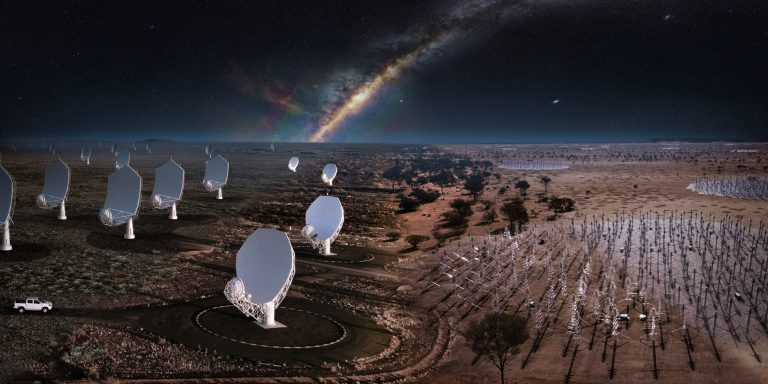
\includegraphics[width=\textwidth]{SKA-at-Night-768x384.jpg} \\
\vspace{0.5cm}
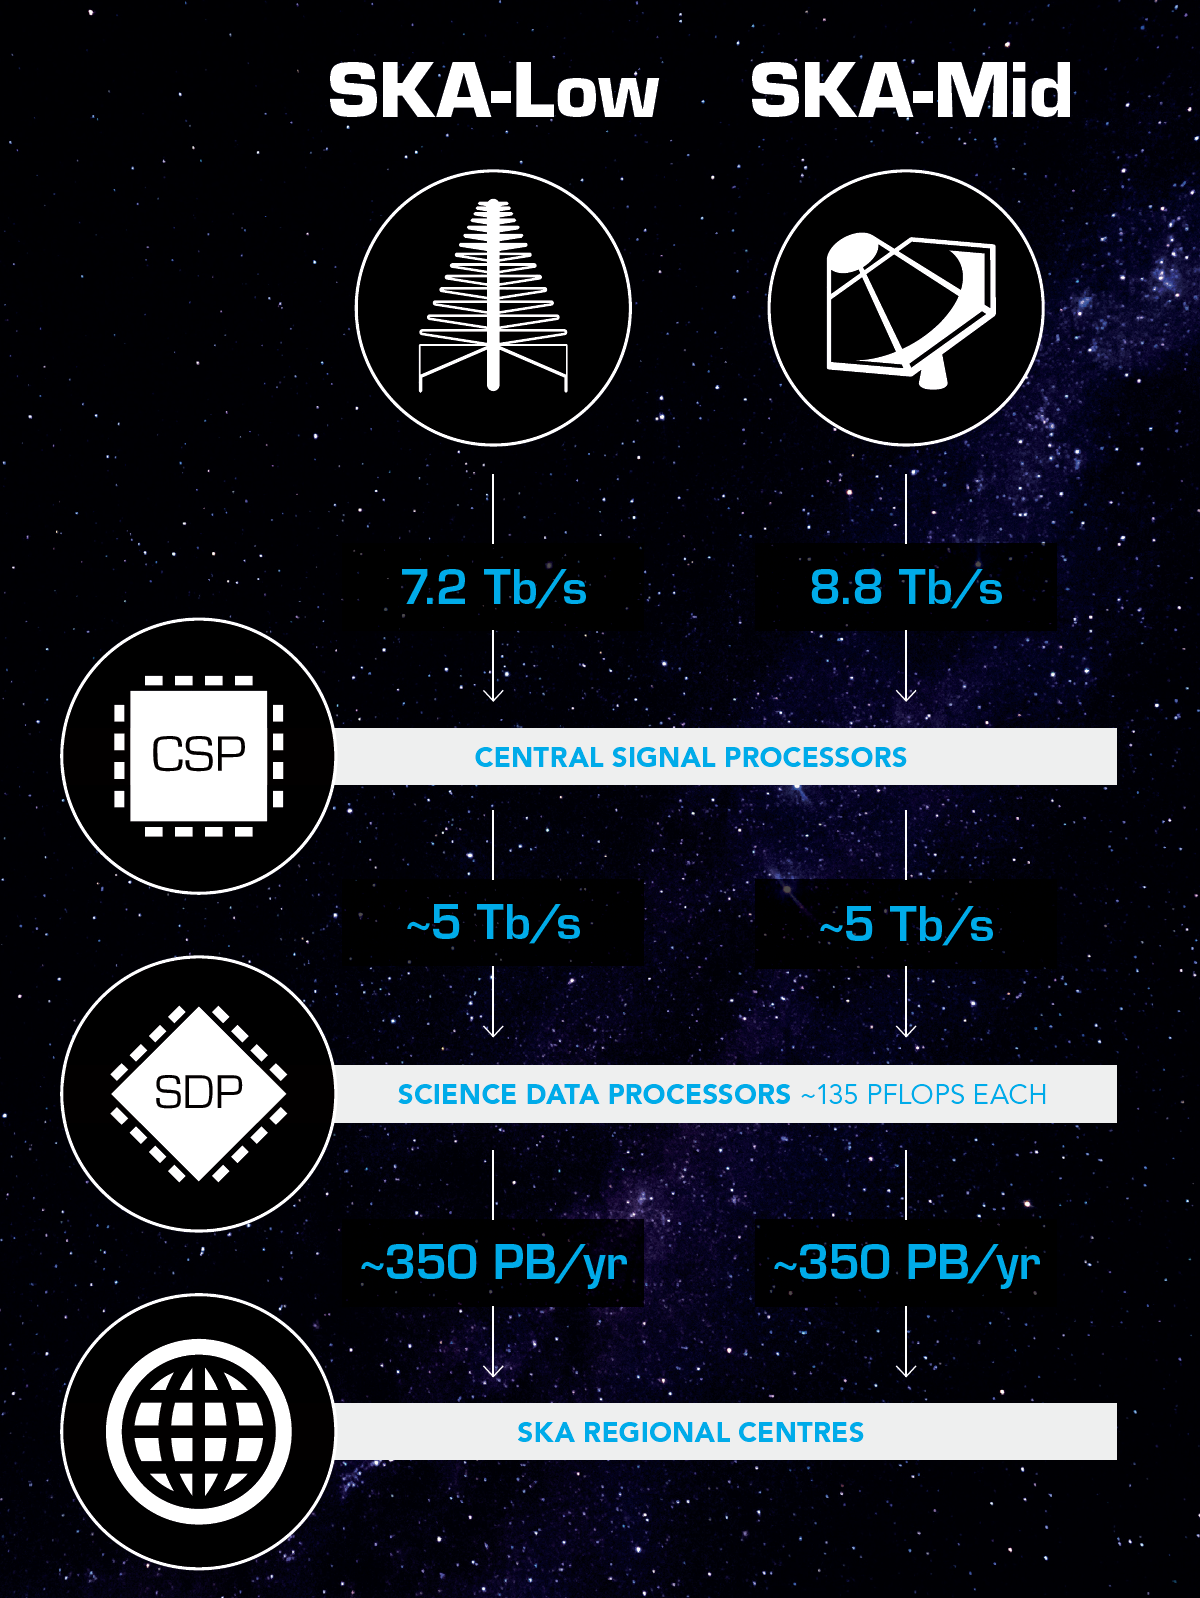
\includegraphics[width=0.7\textwidth]{image002}
\end{center}
\end{column}
\begin{column}{.6\linewidth}
    \begin{block}{Largest radio telescope array ever constructed}
          \begin{itemize}
            \item \textcolor{blue}{200+} dishes in South Africa
            \item \textcolor{blue}{130 000+} antennas in Australia
            \end{itemize}
        \end{block}

            \begin{block}{An imaging pipeline made of three HPC stages}
            \begin{itemize}
                \item[CSP] Antenna voltages correlated to produce \textbf{visbilities} 
                \item[SDP] \textbf{hypercubes} \textit{(sky images at different frequencies)} recontructed from visibilities
                \item[SRC] Post-treatement by regional supercomputers
                \end{itemize}
    \end{block}
   

\end{column}
\end{columns}

   
}
}

\subsection{SKA computing, an HPC challenge}
\frame{
  %  \frametitle{}
%\scriptsize{

    \begin{block}{SDP supercomputer}
        \begin{itemize}
            \item Huge computing requirements to process a \textbf{realtime streaming data} %, \textit{nr. 7.2 Tb/s}
            \item \textbf{Limited energy budget}, \textit{nr. 1 MW for each SDP} 
            \item \textbf{Huge algorithm model gap} between programming langues used by astronomers and HPC developpers, \textit{Python vs MPI/CUDA/...}
        \end{itemize}
       % $\implies$ Challenge to design a power-efficient supercomputer using low power coprocessors for the intensive computing
    \end{block}
    \begin{block}{A \textbf{software/hardware co-design} challenge}<2>
       % Need for time and energy performance assessments 
        \begin{itemize}
            \item New complex scientific \textbf{dataflow algorithms}
            \item Not-yet-existing \textbf{large scale heterogeneous} computing platform
        \end{itemize}
       $\implies$ Call for rapid prototyping tools providing \textbf{early time and energy performance assessments}
    \end{block}
   
%}
}

\section{Dark-era goals}
\frame{
  %  \frametitle{}
%\scriptsize{
   
    \begin{block}{Dark-era goals}
        \begin{enumerate}
            \item Building \textbf{SimSDP, a rapid prototyping tool} providing exascale simulations from dataflow algorithm descriptions.
            \item Exploring \textbf{low power accelerators} like FPGA or Kalray MPPA as alternatives to mainstream GPU architecture.
            \item Contribute to SKA computing challenge
\end{enumerate}
\end{block}

\centering
    %\frametitle{An interdisciplinary Team}
    \begin{block}{SimSDP}<2>
        \centering
    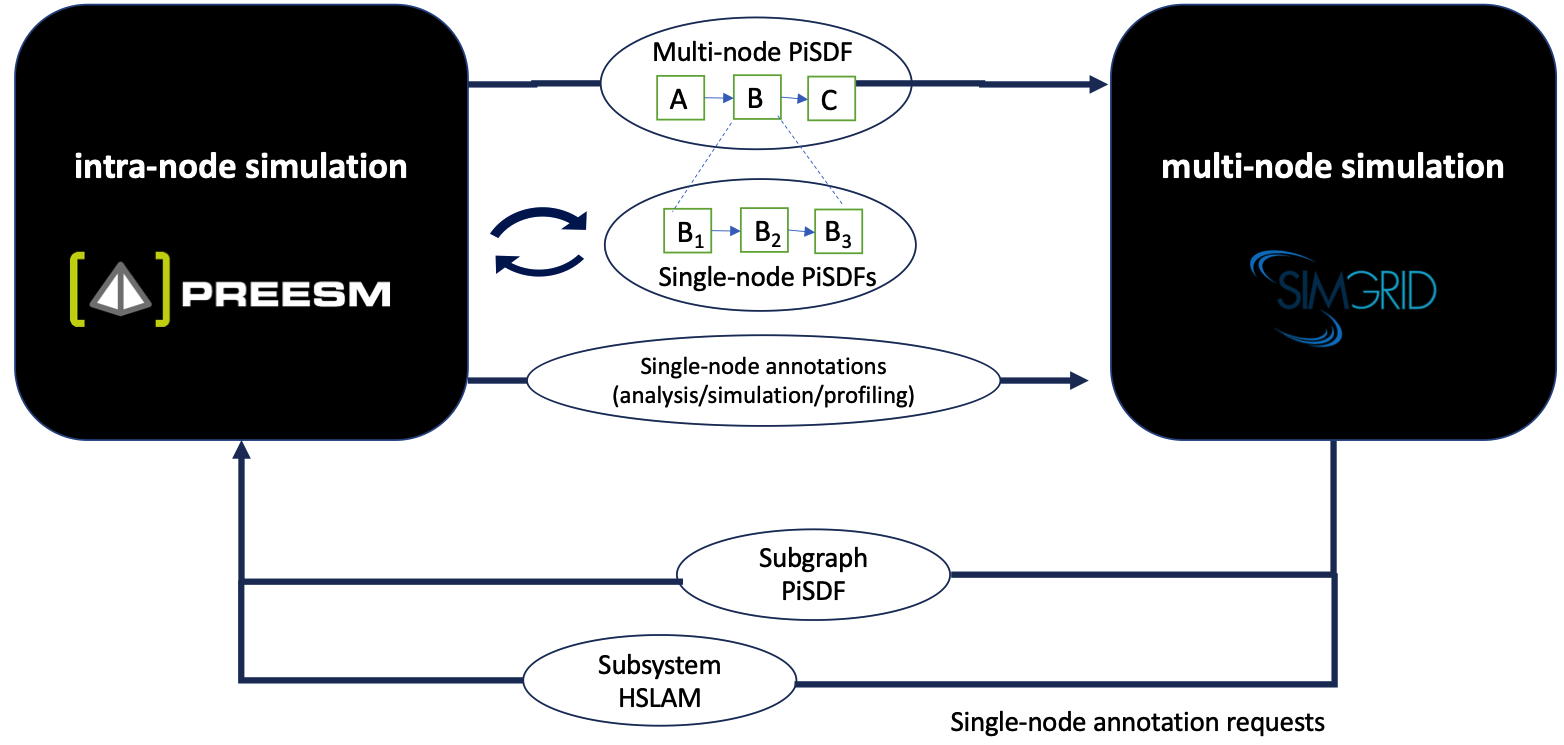
\includegraphics[width=0.75\textwidth]{simsdp_architecture-light.png}  
\end{block}

}


%The \textbf{SDP supercomputer} will be based on a standard HPC system combined with FPGA or application-specific architectures like GPU or the manycore Kalray Massively Parallel Processor Array (MPPA). One crucial challenge is to assess the performance both in time and energy of new complex scientific \textbf{dataflow algorithms} on not-yet-existing complex computing infrastructures. It will be hardly possible without efficient \textbf{co-design methods} and \textbf{rapid prototyping tools}.




\section{Project organisation}


\subsection{Team}


\frame{
    \centering
    \vspace{0.1cm}
    
\includegraphics[width=0.2\textwidth]{DARKERA_logo_color_L}  \\
    \centering
    \vspace{-0.7cm}
    %\frametitle{An interdisciplinary Team}
    %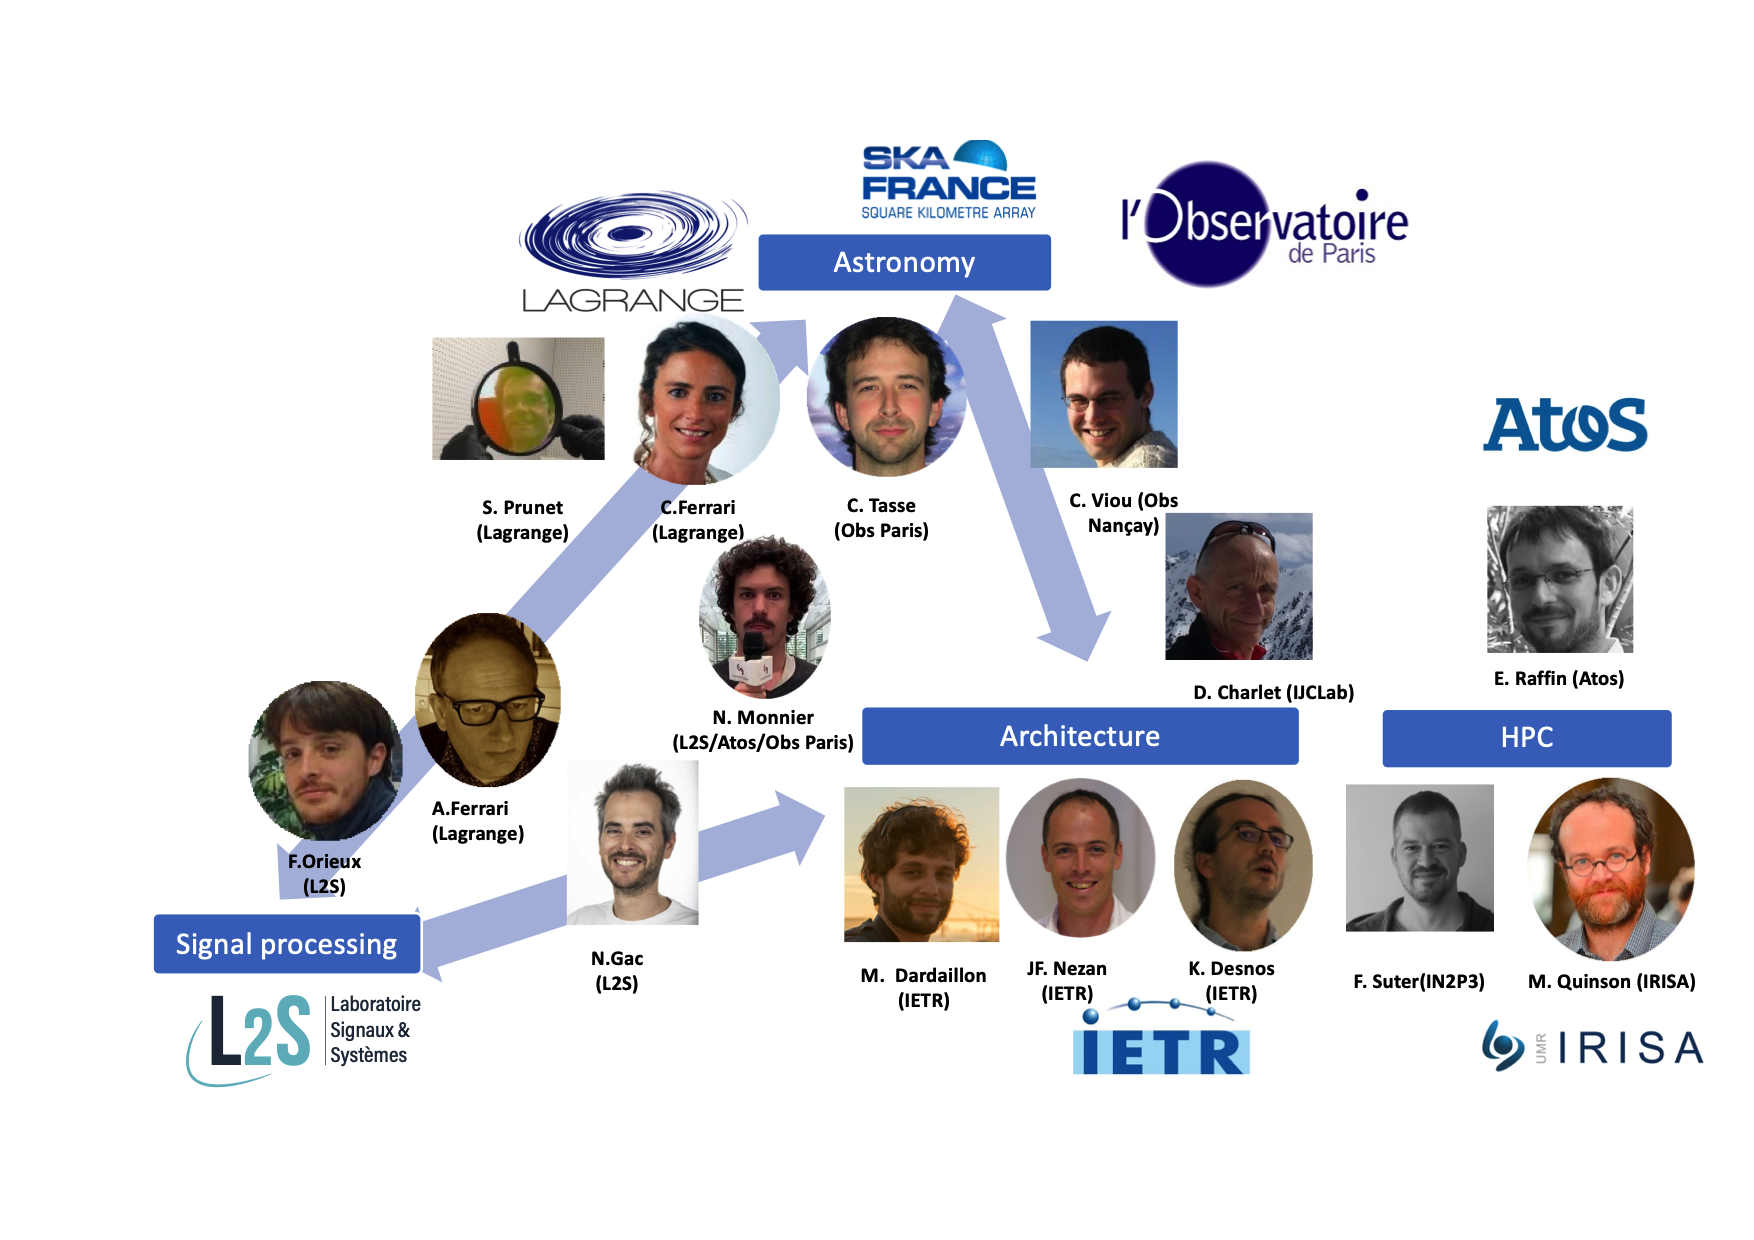
\includegraphics[width=\textwidth]{team-dark-era.png} 
}



\setbeamercolor{background canvas}{bg=black}
\section*{End}
\frame[t,noframenumbering]
{
  
%\frametitle{Projet ANR DARK-ERA (2/2)}
\vspace{2.1cm}
\centering
{\huge\textcolor{white}{More information on the project website :}\\
\vspace{1cm}
\href{https://dark-era.pages.centralesupelec.fr}{\textcolor{white}{https://dark-era.pages.centralesupelec.fr}}\\
\vspace{1cm}
\small{\textcolor{white}{\underline{contact}: nicolas.gac@l2s.centralesupelec.fr}}
}

}


\end{document}

